\documentclass[12pt, a4paper]{article}
\usepackage[utf8]{inputenc}
\usepackage{amsmath}
\usepackage{amsthm}
\usepackage{amssymb}
\usepackage{graphicx}
\usepackage{parskip}
\usepackage{hyperref}
\usepackage{fancyhdr}
\usepackage{lastpage}
\usepackage[vlined,ruled]{algorithm2e}
\usepackage[acronym]{glossaries}
\usepackage{caption}
\usepackage{titlesec}
\usepackage{tikz}
  

\title{%
  Algorithmic Game Theory \\
  Final Exam
}
\author{%
  Juan Pablo Royo Sales\\
  \small{Universitat Politècnica de Catalunya}
}
\date\today

\pagestyle{fancy}
\fancyhf{}
\fancyhead[C]{}
\fancyhead[R]{Juan Pablo Royo Sales - UPC MIRI}
\fancyhead[L]{AGT - Final Exam}
\fancyfoot[L,C]{}
\fancyfoot[R]{Page \thepage{} of \pageref{LastPage}}
\setlength{\headheight}{15pt}
\renewcommand{\headrulewidth}{0.4pt}
\renewcommand{\footrulewidth}{0.4pt}

\renewcommand{\qedsymbol}{$\blacksquare$}
\newacronym{ncg}{NCG}{Network Congestion Game}
\newacronym{sncg}{SNCG}{Symmetric Network Congestion Game}
\newacronym{pne}{PNE}{Pure Nash Equilibrium}
\newacronym{ne}{NE}{Nash Equilibrium}
\newacronym{mincost}{MINCOST}{Min-Cost Flow Problem}
\newacronym{ds}{Dominant Set}{Dominant Set}
\newacronym{sg}{Simple Game}{Simple Game}
\newacronym{is}{IsStrong}{IsStrong}
\newacronym{ip}{IsProper}{IsProper}
\newacronym{mis}{Maximal Independent Set}{Maximal Independent Set}
\newacronym{mvc}{Minimal Vertex Cover}{Minimal Vertex Cover}

\begin{document}

\maketitle

\section{Exercise 1}
A \acrfull{ncg} is \textbf{symmetric} when $s_i = s$ and $t_i = t$, for $i \in N$ according to the definition that we have seen in class. Basically all the players, have the 
same source and destination endpoint $s$ and $t$ and all have the same path strategies.

The algorithm to find \acrfull{pne} in \acrshort{sncg} in \textit{poly-time} is doing a reduction to \acrfull{mincost}
in order to find the Optimum of $\varphi(s)$.

\begin{algorithm}[H]
  \SetKwInOut{Input}{Input}
  \SetKwInOut{Output}{Output}
  \Input{$G = (V, E, s, t)$, $d_e$ delay function}
  \Output{\acrshort{mincost} representation of the problem}
  \For{each $e \in E$}{
    \For{$1$ up to $d_e$}{
      $E \leftarrow E \cup \{e'_i\}$ such that $d_{e'_i} = 1$;\\
    }
    $E \leftarrow E \setminus \{e\}$;\\
  }
  return $N$;
  \caption{Compute \acrshort{mincost} reduction of \acrshort{sncg}}
\end{algorithm}

Basically the reduction is replacing each edge $e$ with the amount of the delay function for $e$ $d_e$ of new edges
but this time each of this edges with delay function equal to $1$.

The \acrshort{mincost} of the new network $N$ minimizes $\varphi(s)$.

Since the algorithm is giving also a Local Optimum, then $s$ is a \acrshort{pne}.

Based on this~\cite{ne_complex}
\section{Exercise 2}
As we have seen in class the \textbf{Social Cost} is the sum of all players 

\begin{equation}
  C(s) = \sum_{u \in V} c_u(s) = \alpha|E| + \sum_{u,v \in V} d_G(u,v)
\end{equation}

Every pair of vertices that is not \textit{connected} its distances is $\ge 2$, there is a lower bound for the 
social cost:

\begin{subequations}
  \begin{align}
    C(s) &\geq \alpha|E| + 2|E| + 2(n(n - 1) - 2|E|)\\
         &= 2n(n - 1) + (\alpha - 2)|E|\label{eq:1}
  \end{align}
\end{subequations}

\subsection{(a)}
In this case when $\alpha < 1$ the social Optimum is achieved when $|E|$ is maximum. So, every vertex is connected with each other. It is a complete graph.
Any \acrfull{ne} should be of diameter $1$ which implies that the complete graph is the only \acrshort{ne}.

\subsection{(b)}
In the case $1 \leq \alpha < 2$, the social Optimum is achieved by a complete graph, but not \acrshort{ne}. Any \acrshort{ne} is for diameter at most $2$.
So, the social cost is equal to~\ref{eq:1} and it is the worst cost when $|E|$ is minimum, which is $n-1$ for a connected graph. Therefore the worst \acrshort{ne} is the $S_n$ Star.

\subsection{(c)}
As we have seen in class when $\alpha > 2$ we need to minimize the number of edges $|E|$ in order to reduce the cost, but at the same time the graph should be connected.
Therefore only trees with diameter $2$ have optimal cost. One example that has \acrshort{ne}, with diameter $2$ and minimum number of edges is a \textbf{Cycle Graph} with 4 vertex.

\subsection{(d)}
Since when $\alpha > n^2$ no player has any incentive to buy an edge, there is going to be the minimum amount possible of edges at the same time with the graph connected, 
that by definition are \textbf{Spanning Trees} as we have seen in class. All are \acrshort{ne} because no one has incentive to change.
The $PoA$ is giving by:

\begin{subequations}
  \begin{align}
    PoA &= \frac{c(T_n)}{c(S_n)}\\
        &\leq \frac{\alpha(n-1)+(n-1)(n-1)}{\alpha(n-1)+1+2n(n-1)}\\ 
        & = O(1)
  \end{align}
\end{subequations}

Based on this~\cite{network_creation}.

\section{Exercise 3}
\subsection{(a)}
In order to show that it is a \acrfull{sg}, we need to show that the valuation function is \textbf{monotone}.

We assume in this game that

\[ v(X) = \begin{cases}
  1 \textit{ if X is a \acrlong{ds} set of G}\\
  0 \textit{ otherwise}
\end{cases}
\]

And on the other hand we know that A Game is monotone if $v(C) \leq v(D)$ for any $C, D$ such that $C \subseteq D$.

Lets take any $C,D \in G$ such that $C \subseteq D$ and lets consider the following cases:

\begin{itemize}
  \item If $D$ is a \acrfull{ds}, any subset of vertices on $D$, lets call $C$ such that $C \subseteq D$, have 2 possibilities: either
  \begin{itemize}
    \item $C$ is also dominant because we remove some border vertex which adjacency vertices are connected to other $v \in C$, so $v(C) = v(D) = 1$
    \item $C$ is not dominant because selected subset is not a resulting \acrlong{ds}, in which case $v(C) = 0 < v(D)$
  \end{itemize}
  \item If $D$ is non dominant then any subset is also non dominant so $v(C) = v(D) = 0$.
\end{itemize}

Then we can conclude that $v(C) \leq v(D)$, for any $C, D \in G, C \subseteq D$. So this is \textbf{monotone}.

Therefore it is a \acrshort{sg}.

\subsection{(b)}
Base on the theorem that states \textit{A simple game has non-empty core if and only if it has a veto player}, we can check
if there is a veto player for some \textit{dominant game} in order to see if it has a non-empty core.
An example of that is a $S_n$ star in which the center vertex $c$ belongs to any coalition that contains $c$ but it cannot be remove from any of those 
coalition because if we remove it it is not a \acrlong{ds}.

\subsection{(c)}
Lets analyze case by case. We are going to analyze \acrshort{is} and \acrshort{ip}

\subsubsection{IsProper Analysis}
A Game $\Gamma$ is proper if $S \in W \implies N \setminus S \notin W$.

Let $S \in W$, then for every vertex $u \in S$, we have the following cases:
\begin{itemize}
  \item $u \notin N \setminus S$, but that not implies that $N \setminus S \notin W$, because it can be another \acrlong{ds}.
  For example if we have an cycle square connected in each vertex, and $S$ are 2 adjacent vertices. $N \setminus S$ is still another $W$. 
  In that case the game is not proper. Let see an example

  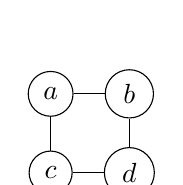
\begin{tikzpicture}[main/.style = {draw, circle}] 
    \node[main] (1) {$a$}; 
    \node[main] (2) [right of=1] {$b$}; 
    \node[main] (3) [below of=1] {$c$}; 
    \node[main] (4) [below of=2] {$d$}; 
    \draw (1) -- (2);
    \draw (1) -- (3);
    \draw (2) -- (4);
    \draw (3) -- (4);
  \end{tikzpicture} 

  As we can see here for example if $\{a,b\} \in S$ which $\in W$, but the complement which is $\{b,d\} \in W$ as well.

  \item In order $N \setminus S \notin W$ we need that all $u \in W$ form a single Coalition. That means that $S$ should be a \acrfull{mis},
  because by definition every \acrlong{mis} is a \acrlong{ds}. In that case the Game is proper.
\end{itemize}

Therefore in order to analyze if the Game \acrlong{ip} we need to provide an algorithm that check if the provided $S$ is a \acrlong{mis}.
Such an algorithm can be computed in \textit{poly-time} because it is known that finding a \acrlong{mis} can be done in \textit{poly-time} according to this~\cite{mis_complex}.
Once we have the \acrlong{mis} of $G$, we need to check for each $u \in S$ if it is belongs to the \acrlong{mis}.

\begin{algorithm}[H]
  \SetKwInOut{Input}{Input}
  \SetKwInOut{Output}{Output}
  \Input{$G = (V, E)$, $S$}
  \Output{$S$ IsProper}
  $MIS \leftarrow$ \textbf{Compute \acrlong{mis} in \textit{poly-time}}\\
  \For{each $u \in S$}{
    \If{$u \notin MIS$}{
      return Not Proper;\\
    }
  }
  return IsProper;
  \caption{Compute if $S$ IsProper}
\end{algorithm}

\subsubsection{IsStrong Analysis}
A Game $\Gamma$ is strong if $S \notin W \implies N \setminus S \in W$.

Let $S \notin W$, then for every vertex $u \in S$, we have the following:
\begin{itemize}
  \item $u \notin N \setminus S$, but that not implies that $N \setminus S \in W$, because it can be another subset that is $\notin W$.
  In that case the game is not strong. Let see an example

  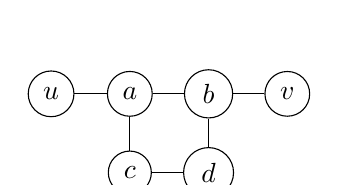
\begin{tikzpicture}[main/.style = {draw, circle}] 
    \node[main] (1) {$a$}; 
    \node[main] (5) [left of=1] {$u$}; 
    \node[main] (2) [right of=1] {$b$}; 
    \node[main] (3) [below of=1] {$c$}; 
    \node[main] (4) [below of=2] {$d$}; 
    \node[main] (6) [right of=2] {$v$}; 
    \draw (1) -- (2);
    \draw (1) -- (3);
    \draw (1) -- (5);
    \draw (2) -- (4);
    \draw (3) -- (4);
    \draw (2) -- (6);
  \end{tikzpicture} 

  As we can see here for example if $\{a,b,u\} \in S$ which $\notin W$, but the complement which is $\{b,d,v\} \notin W$ as well.

  \item In order $N \setminus S \in W$ we need that all $u \notin W$ are maximal losing form. That means that $S$ should be a \acrfull{mvc},
  because by definition we know that the complement of \acrlong{mis} is a \acrlong{mvc}. In that case the Game is proper.
\end{itemize}

It is well known that \textbf{decision Problem} for \textbf{Vertex Cover} is \textit{NP-Complete} for an arbitrary graph.
So \acrlong{is} is $NP-hard$ at least for deciding whether or not $S$ is a \acrlong{mvc}.

\subsection{(d)}
Given the fact as we have explained before we can calculate \acrfull{mis} in \textit{poly-time}, 
we can build a \textbf{Minimum Dominant Set} starting from the \acrshort{mis} and removing vertex checking that we still have
an \acrlong{ds}. 
But the issue with that is that we can have exponential number of possible ways of removing or combining the removal process from the \acrlong{mis}.
So the problem is in \textit{NP}, since we have different decision trees on the removal process.

\section{Exercise 4}
\subsection{(a)}
\newtheorem{case_a}{}
\newtheorem{proofpart_a}{Part}
\begin{case_a}
  A candidate $a$ can win an election at node $u \in T \iff a$ can win in $1$ of $u$'s children subelections and it can defeat one 
  of the potential winner of other sibling child of $u$ in a pairwise election.
\end{case_a}

\begin{proof}
  \begin{proofpart_a}
  $\implies$\\
  This part is trivial because of the structure of the Balance Tree.
  \end{proofpart_a}

  If we take lets say this candidate $a$ and this can win an election at node $u \in T$, we can think on that subtree which root is $a$ that $a$ is the winner of that subtree according to Cup definition.

  Then if it is the winner it is because it should win in some sub-children pairwise election in order to appear at the top.

  Since that $a$ belongs to a subtree of $T$ that subelections that wins should be for some of the subchildren of $T$.

  Also it is trivial that $a$ defeat any other sibling of $u$ otherwise it shouldn't be at the root of this subtree.
  
  \begin{proofpart_a}
  $\impliedby$\\
  This part is not so trivial and we need to do it in two subparts.\\
  \begin{enumerate}
    \item If $a$ can win in $1$ of $u$'s children subelections of $T$
    \item If $a$ can defeat one of the potential winner of other sibling child of $u$ in a pairwise election.
  \end{enumerate}
  If $1 \land 2 \implies a$ can win an election at node $u \in T$.
  \end{proofpart_a}

  \begin{itemize}
    \item Lets assume that point $1$ holds, and $a$ competes in a pairwise election with some $b$ candidate in a subelection of $T$. 
    If that happens and $a$ wins to $b$ the parent node of $a$ and $b$ would be $a$.
    \item At the same time in other sibling of $u$ tree could be an election of in which there could be a potential winner lets say $c$. 
    At some point that $c$ are going to compete with $a$ because they are going to raise to the tree roots. If that happens and as the problem 
    state, if $a$ can defeat this potential winner $c$, then $a$ continue to the root and not $c$.
  \end{itemize}

  Therefore, $a$ can win an election at node $u \in T$.
\end{proof}

\subsection{(b)}
Since the voters in $T$ should form a coalition in order to raise to the top to the tree the candidate $p \in A$, the idea of the algorithm
is that this coalition manipulate elections in the leafs for those candidates that can be defeated by $p$ in pairwise elections, constructing the pairwise competition
in such a way that they can raise $p$ to compete with the worst candidates. This basically can be done with a version of CSL algorithm~\cite{csl} but in a bottom up version instead of top down, and it takes $O(n^2)$

The algorithm is as following:

\begin{algorithm}[H]
  \SetKwInOut{Input}{Input}
  \SetKwInOut{Output}{Output}
  \Input{$p \in A$ pref candidate, $T$ Manipulator, $C$ Binary Tree, $D$ assignment of leaves}
  \Output{True if $p$ can win via manipulation, False otherwise}
  $MW \leftarrow $ConstructWinnersCCM(T,C,D)
  \If{$p \in MW$}{
    return True;
  }\Else{ return False; }
  \caption{Compute CCM over $p \in A$}
\end{algorithm}

\begin{algorithm}[H]
  \SetKwInOut{Input}{Input}
  \SetKwInOut{Output}{Output}
  \Input{$T$ Manipulator, $C$ Binary Tree, $D$ assignment of leaves}
  \Output{Winner Set Manipulated}
  \If{isLeaf(C)}{
    return $\{C\}$;
  }\Else{
    $W \leftarrow \{\}$\tcp*[r]{Possible Winner Set}
    \textbf{leftTree} $\leftarrow$ ConstructWinnersCCM(T, Left(C), D);\\
    \textbf{rightTree} $\leftarrow$ ConstructWinnersCCM(T, Right(C), D);\\
    \ForAll{$u \in leftTree$}{
      \If{$\exists v \in rightTree$ such that $(u,v) \in D \lor v \in T$}{
        $W \leftarrow \{u\}$
      }
    }
    \ForAll{$v \in rightTree$}{
      \If{$\exists u \in leftTree$ such that $(v,u) \in D \lor u \in T$}{
        $W \leftarrow \{v\}$
      }
    }
    return $W$;
  }
  \caption{ConstructWinnersCCM(T,C,D)}
\end{algorithm}

Based on this~\cite{ccmalgo}.

\bibliographystyle{alpha}
\bibliography{jproyo_final_exam}
\end{document}